% !TEX root = ../Thesis.tex

\chapter{Integrazione di OpenNebula con FACPL}
\label{cap:proposal}
Come già discusso nel capitolo \ref{cap:stateOfArt}, grazie al modo in cui FACPL\cite{facpl} è costruito risulta molto facile andare a fornire un'implementazione concreta dei PEP (\emph{Policy Enforcement Point}) e PDP (\emph{Policy Decision Point}) avendo conoscenza  di quali sono le esigenze a cui devono rispondere.\medbreak
Per validare ulteriormente questo punto abbiamo deciso di utilizzare FACPL in una situazione in cui fosse necessario interfacciarsi con un software già esistente così da mostrare le effettive potenzialità e semplicità di implementazione della libreria.
Il caso concreto che abbiamo deciso di considerare deriva da un possibile sviluppo futuro già proposto all'interno di \cite{10.1007/978-3-319-08260-8_6}, ovvero un'integrazione con un "sistema di IaaS open-source sul cloud" come OpenNebula\cite{opennebula}, software che è stato già presentato all'interno del capitolo \ref{cap:stateOfArt}.

\section{Idea di base}
Per iniziare abbiamo considerato due esempi di gestione delle risorse disponibili aderenti alla realtà, presenti all'interno di \cite{10.1007/978-3-319-08260-8_6}.
Abbiamo inoltre potuto osservare due primi tentativi di implementazione descritti sempre all'interno di \cite{10.1007/978-3-319-08260-8_6}:
\begin{itemize}
    \item il primo sviluppato basandosi su una completa astrazione, ovvero dei files che simulano un sistema con diverse virtual machine, che è presente anche in \cite{facpl-github} fra gli esempi nella cartella \emph{EXAMPLES}.
    \item il secondo basato su uno XEN Hypervisor, che però non è presente fra gli esempi forniti assieme alla libreria e di cui non vengono esplicitati i dettagli di implementazione.
\end{itemize}
Con questa conoscenza l'obiettivo iniziale è stato quello di riuscire ad interagire con un reale sistema su cui è installato un cloud manager per fare si che questo eseguisse i comandi necessari per eseguire le PEP action da noi richieste e ci esponesse tutte le informazioni necessarie al PDP per valutare le richieste.
Nel concreto era quindi necessario pensare a due parti distinte:
\begin{itemize}
    \item una che svolgesse operazioni sulle singole virtual machine (avviarle, inserire nell'host corretto, fermarne l'esecuzione).
    \item una che recuperasse le informazioni generali sugli host e sul sistema tutto.
\end{itemize}
Il cloud manager che abbiamo deciso di utilizzare è stato OpenNebula per i motivi presentati nel capitolo \ref{cap:stateOfArt}

\section{OpenNebula API}
Il primo approccio che avevamo pensato di percorrere era quello di utilizzare il codice Java per invocare dei comandi da shell che fossero in grando di interagire con OpenNebula. Questo approccio sembrava il più immediato anche dato lo studio preliminare di OpenNebula che avevamo svolto che era stato soprattutto attraverso la shell (oltre che la web ui).\medbreak
Per utilizzare i comandi da shell che permettono di interagire con OpenNebula occorre aver effettuato l'autenticazione come utente OpenNebula\footnote{\url{https://docs.opennebula.io/6.8/management_and_operations/users_groups_management/manage_users.html}}.
Questa soluzione aveva il principale vantaggio di poter fornire un'interfaccia generica che permettava in un futuro di far interagire con sforzo minimo FACPL anche con comandi di natura completamente diversa, tuttavia presentava anche diverse problematiche come la forte dipendenza dalla versione di OpenNebula installata nel sistema e una grande inefficienza nello svolgimento di alcune operazioni, oltre che alcune difficoltà in fase di test.\medbreak
La strada su cui ci siamo orientati è stata quindi quella di utilizzare le API di OpenNebula per Java\footnote{\url{https://docs.opennebula.io/6.8/integration_and_development/system_interfaces/java.html}} in quanto queste semplificavano l'ottenimento di alcune informazioni. Come è possibile leggere dal sito di OpenNebula stesso, queste API sono a loro volta un wrapper dei metodi XML-RPC\footnote{\url{https://docs.opennebula.io/6.8/integration_and_development/system_interfaces/api.html\#api}}.
Le API utilizzate sono quelle della versione 5.12.0\footnote{\url{https://downloads.opennebula.io/packages/opennebula-5.12.0/}} dato che dopo la major version 5 sono compilate con la versione di Java 11 (al contrario di quato riportato sul sito stesso) e di conseguenza non erano compatibili con la versione di Java 8 con cui è stato sviluppato FACPL.
I principali attori che sono stati utilizzati dalle API\footnote{\url{https://docs.opennebula.io/doc/6.4/oca/java/org/opennebula/client/package-summary.html}} sono stati:
\begin{itemize}
    \item \emph{Client}: è la classe principale che gestisce la connesione fra il core di OpenNebula e le chiamate XML-RPC, quasi tutti gli altri oggetti delle API richiedono di passare un oggetto di questo tipo per poter essere istanziati. Questo oggetto può essere istanziato passando uno \emph{username} e una \emph{password} al costruttore, ma presenta anche un costruttore che non richiede parametri e permette di derivare \emph{username} \emph{password} dall'utente corrente.
    \item \emph{ClientConfigurationException}: è la classe che rappresenta l'eccezione che viene lanciata se si tenta di istanziare un \emph{Client} con delle impostazioni di autorizzazione sbagliate, in particolare se \emph{username} \emph{password} sono errate oppure se si tenta di usare il costruttore vuoto lanciando il programma da un utente che non è uno user di OpenNebula.
    \item \emph{OneResponse}: è la classe che incapsula le risposta XML-RPC di OpenNebula, viene istanziata con un \emph{boolean} e una \emph{String} che rappresentano rispettivamente l'esito della richiesta (positivo o negativo) e un eventuale messaggio che lo descrive. Quasi tutte le azioni eseguibili sui \emph{PoolElement} ritornano un oggetto di questo tipo.
    \item \emph{Pool}: è la classe che rappresenta un insieme di \emph{PoolElement} e fornisce la possibilità di scorrere gli stessi ed eseguire in modo agevolato alcune operazioni
    \item \emph{PoolElement}: è la superclasse della maggior parte delle classi che rappresentano gli elementi di OpenNebula, quelli più interessati nel progetto sono stati
          \begin{itemize}
              \item \emph{VirtualMachine}
              \item \emph{Host}
              \item \emph{Template}
          \end{itemize}
\end{itemize}

\section{Logging}
Prima ancora di pensare ai comandi da eseguire sulle virtual machine si è reso necessario pensare ad una modalità di logging. Dato l'ambito di applicazione si è resa fondamentale la scrittura di logs su file di modo da rendere gli stessi facilmente accessibili in futuro, anche a distanza di tempo.\medbreak
All'interno del progetto è quindi fornita una classe \texttt{FileLoggerFactory} che utilizza il design pattern \emph{Static Factory Methods} \cite{effectiveJava} e permette di creare dei file di log, di modo da evitare la necessità di interagire coi file in ogni classe che intende eseguire il log di informazioni oltre che gestire in modo consono gli handler dei files evitando duplicati. Questa classe permette di creare dei \texttt{Logger} con un'implementazione di \texttt{Level} e \texttt{Formatter} di default oppure di specificare questi parametri in input.
\begin{lstlisting}[language=Java, caption={Metodo make di FileLoggerFactory}, label=code:FileLoggerFactoryMake]
public static Logger make(String fileName, Formatter formatter, Level level) {
    Throwable t = new Throwable();
    StackTraceElement directCaller = t.getStackTrace()[1];
    String loggerName = directCaller.getClassName() + "-" + fileName;

    Logger logger = Logger.getLogger(loggerName);

    @+\mytikzmark{hl1Start}@+if (!isFileHandlerAttached(logger, fileName)) {@+\mytikzmark{hl1End}@+
        try {
            FileHandler fileHandler = createFileHandler(fileName, formatter, level);
            logger.addHandler(fileHandler);
            logger.setUseParentHandlers(false);
        } catch (IOException e) {
            throw new RuntimeException("Failed to initialize logger handler.", e);
        }
    @+\mytikzmark{hl2Start}@+}@+\mytikzmark{hl2End}@+

    return logger;
}
    \end{lstlisting}
\begin{tikzpicture}[remember picture, overlay]
    \highlight{hl1Start}{hl1End}
    \highlight{hl2Start}{hl2End}
\end{tikzpicture}
Nonostante la presenza di questa classe, tutte le classi all'interno del progetto hanno i logger passati tramite dependency injection e forniscono un'implementazione di default che esegue logging nello standard output (solitamente la console). L'unica classe che fa eccezione in questo è proprio \texttt{ContextStub\_Default} che è il primo punto di ingresso della dipendenza.\\
L'idea è che nel caso in cui si preferisca eseguire logging in modo diverso si possa definire un logger diverso al posto dell'implementazione proposta. Per farlo occorre semplicemente modificare una riga all'interno del costruttore di \texttt{ContextStub\_Default}:
\begin{lstlisting}[language=Java, caption=Costruttore ContextStub\_Default, label=code:CostContextStub]
public static ContextStub_Default getInstance() {
    if (instance == null) {
        try {
            Configuration config = new Configurations().properties(CONFIG_FILE);
            hyper1HostId = config.getString("hyper1.host.id");
            hyper2HostId = config.getString("hyper2.host.id");
            ContextStub_Default.oneClient = new Client();
            @+\mytikzmark{hl1Start}@+Logger logger =@+\mytikzmark{hl1End}@+ @+\mytikzmark{hl2Start}@+FileLoggerFactory.make("logs/virtualMachines.log");@+\mytikzmark{hl2End}@+				inizializeStub(oneClient, logger);
            instance = new ContextStub_Default();
        } catch (ClientConfigurationException e) {
            throw new RuntimeException("Failed to initialize Client: " + e.getMessage(), e);
        } catch (ConfigurationException e) {
            throw new RuntimeException(
                    "Errors in the config gile: " + e.getMessage(), e);
        } catch (Exception e) {
            throw new RuntimeException(
                    "Unexpected error during ContextStub_Default initialization: " + e.getMessage(), e);
        }
    }
    return instance;
}

\end{lstlisting}
\begin{tikzpicture}[remember picture, overlay]
    \highlight{hl1Start}{hl1End}
    \highlight{hl2Start}{hl2End}
\end{tikzpicture}
\section{Gestione delle virtual machine generiche}
Per gestire le virtual machine l'approccio iniziale è stato quello di fornire un'interfaccia che permettesse in un futuro di poter interagire con le stesse anche in modo diverso.
E' stata creata una classe wrapper chiamata \texttt{VMDescriptor} che contiene le informazioni sulle virtual machine utili per il nostro progetto, questa classe serve per creare una prima astrazione dalle API utilizzate, in effetti questa stessa classe permetterebbe, ad esempio, di fornire un'implementazione come quella precedentemente pensata basata sui comandi da shell.
L'interfaccia \texttt{VirtualMachineService} presenta due metodi che servono per lavorare all'effettivo con i \texttt{VMDescriptor}.
\begin{lstlisting}[language=Java, caption=VirtualMachineService, label=code:VirtualMachineService, xleftmargin=1em]
public interface VirtualMachineService {
    List<VMDescriptor> getVirtualMachinesInfo();
    List<VMDescriptor> getRunningVirtualMachineInfo();
}
\end{lstlisting}
La scelta di avere due metodi separati per restituire tutte le macchine virtuali oppure solo quelle attualmente in esecuzione deriva dal fatto che in effetti spesso queste due liste vorranno essere utilizzate in modo diverso. Di solito le VirtualMachine presenti nel sistema sono molte più di quelle effettivamente in esecuzione e quindi non inserire il secondo metodo avrebbe portato una buona parte delle classi che volevano utilizzare un'implementazione di questa interfaccia a dover sempre inserire un controllo sullo stato delle virtual machine.
Nel codice da me scritto viene utilizzata la sua implementazione concreta \texttt{OpenNebulaVMService} che, interfacciandosi con le API di OpenNebula già descritte, riesce ad ottenere tutte le informazioni richieste sulle virtual machine e a popolare le liste.
Una volta ottenuta una lista di \texttt{VMDescriptor} è possibile filtrare le virtual machine sia a partire dal nome che a partire da altre loro caratteristiche come l'\emph{ID} o il \emph{template} utilizzato per crearle come spiegato nel capitolo \ref{cap:stateOfArt}.
È stata implementata un'ulteriormente classe di comodo che mette a disposizione la possibilità di eseguire alcuni tipi di filtraggio sulle virtual machine in automatico, questa classe fornisce inoltre un meccaniscmo di logging ogni volta che viene eseguita un'operazione di filtraggio, come si può vedere nel codice di esempio:
\begin{lstlisting}[language=Java, label=code:VMsInfoLogging, xleftmargin=1em]
private List<VMDescriptor> getAndLogVMs() {
    List<VMDescriptor> vmDescriptors = vmService.getRunningVirtualMachineInfo();
    logger.info("The VMs running are: " + vmDescriptors.toString());
    return vmDescriptors;
}
\end{lstlisting}
\begin{lstlisting}[language=Java, label=code:VMsInfoFilter, xleftmargin=1em, basicstyle=\fontsize{9}{10}\ttfamily]
public List<VMDescriptor> getRunningVMsByHostTemplate(String host, String templateId) {
    return getAndLogVMs()
            .stream()
            .filter(x -> x.getHostId().equals(host) && x.getTemplateId().equals(templateId))
            .collect(Collectors.toList());
}
\end{lstlisting}
\captionof{lstlisting}{Esempio di metodo di filtraggio e metodo di logging}
Non è necessario usare questa classe, però risulta comoda per fare sì che le classi che si occupano di eseguire un comando su una o più virtual machine non abbiano anche il compito di eseguire il filtraggio e fare logging.

\section{Gestione delle virtual machine di OpenNebula}
Da qui in avanti saranno presentate tutte le classi che interagiscono effettivamente con degli oggetti che rappresentano delle \texttt{VirtualMachine} come indicato nelle API di OpenNebula.
La prima classe implementata è \texttt{OpenNebulaActionContext}, questa classe può essere istanziata usando un \texttt{Client} (e opzionalmente anche un \texttt{Logger}) e fornisce semplicemente uno stato da utilizzare per eseguire i comandi che richiedono informazioni sulle \texttt{VirtualMachine} attualmente in esecuzione, che in questo caso concreto saranno tutti tranne la creazione di una nuova virtual machine.\\
La classe per eseguire i comandi ha la seguente base:
\begin{lstlisting}[language=Java, caption=Classe astratta per i comandi, label=code:OpenNebulaActionBase]
public abstract class OpenNebulaActionBase implements IPepAction{
    protected final OpenNebulaActionContext ONActionContext;

    public OpenNebulaActionBase(OpenNebulaActionContext ONActionContext) {
        this.ONActionContext = ONActionContext;
    }
    
    public abstract void eval(List<Object> args);
    
    protected void logResponse(OneResponse response) {
        if (response.isError()) {
            ONActionContext.getLogger().severe(response.getErrorMessage());
        } else {
            ONActionContext.getLogger().info(response.getMessage());
        }
    }
}
\end{lstlisting}
Per questa classe è stato valutato l'utilizzo di un \texttt{Themplate method}, tuttavia risultava abbastanza scomodo da applicare dato che alcune delle classi concrete potrebbero dover seguire un workflow diverso fra loro (es. sospensione di una virtual machine e creazione di una virtual machine) per il modo in cui le API di OpenNebula sono scritte. Inoltre si suppone la possibilità di scrivere comandi futuri che agiscano su più di una virtual machine in un solo comando, questa logica era già stata testata ma non si è rivelata necessaria nel nostro caso concreto e di conseguenza è stata successivamente rimossa, tuttavia il modo in cui è scritta la classe astratta lascia spazio ad una facile implementazione concreta in questo senso.\medbreak
La scelta del nome \texttt{eval} è obbligata dal modo in cui FACPL accederà alla classe per eseguire i comandi.
L'approccio scelto è quello di costruire l'oggetto di tipo \texttt{VirtualMachine} corrispondente all'\emph{ID} ottenibile dal \texttt{VMdescriptor}. Questo passaggio può sembrare controintuitivo perchè partendo da un oggetto \texttt{VirtualMachine} si ottengono le sue informazioni per poi andare a ricreare un oggetto sostanzialmente identico per eseguire le operazioni, tuttavia questi passaggi hanno diversi lati positivi:
\begin{itemize}
    \item Rendono il codice indipendente dalla modalità con cui si ottengono le informazioni sulle virtual machine
    \item Rendono il codice più aperto a modifiche e future implementazioni
    \item Rendono il codice molto più semplice da testare
    \item Isolano l'ottenimento delle informazioni ad una classe che estende \texttt{OpenNebulaVMService}
\end{itemize}
Le classi concrete per eseguire i comandi sulle virtual machine a partire da questa classe hanno tutte chiaramente una forma simile sebbene con alcuni accorgimenti.
\begin{lstlisting}[language=Java, caption=Classe per avviare una \texttt{VirtualMachine}, label=code:CreateVM, basicstyle=\fontsize{8.5}{9.5}\ttfamily]
public class CreateVM extends OpenNebulaActionBase {
	public CreateVM(OpenNebulaActionContext ONActionContext) {
		super(ONActionContext);
	}

	public void eval(List<Object> args) {
		ONActionContext.getLogger().info("Starting VM: " + "[" + args.get(2) + ", " + args.get(1) + "]");
		Template template = new Template((int) args.get(2), ONActionContext.getClient());
		OneResponse instantiateResponse = template.instantiate((String) args.get(1));
		logResponse(instantiateResponse);
		if (!instantiateResponse.isError()){
			VirtualMachine vm = 
					new VirtualMachine(instantiateResponse.getIntMessage(), ONActionContext.getClient());
			logResponse(vm.deploy((int) args.get(0)));
		}		
	}
}
\end{lstlisting}
La classe \texttt{CreateVM}, utilizza un oggetto di tipo \texttt{Template}, che, come già anticipato all'interno del capitolo \ref{cap:stateOfArt} permette di definire le caratteristiche per la creazione di una specifica virtual machine. Nel nostro caso concreto l'oggetto template risulta utilissimo per fare sì che la definizione delle caratteristiche delle virtual machine da utilizzare sia fatta attraverso la UI di OpenNebula (o comunque con dei file appositi validati da OpenNebula tramite UI o comando da shell). Nel caso di studio\footnote{\cite{10.1007/978-3-319-08260-8_6}} vengono considerati due tipi di virtual machine istanziabili, quindi nei nostri test abbiamo spesso considerato due template che fossero in grado di riprodurre i comportamenti richiesti, tuttavia grazie al \texttt{Template} si apre la strada all'utilizzo di virtual machine dalle caratteristiche più disparate senza neanche bisogno di cambiare il codice Java. Infatti grazie al modo in cui è scritto il codice basta definire in OpenNebula un nuovo template e utilizzare il suo ID all'interno di policy e richieste FACPL per poter creare (o distruggere, frezzare ecc.) delle virtual machine di quel tipo.\medbreak

\begin{lstlisting}[language=Java, caption=Classe per freezzare(sospendere) una \texttt{VirtualMachine}, label=code:FreezeVM, basicstyle=\fontsize{8.5}{9.5}\ttfamily]
public class FreezeVM extends OpenNebulaActionBase {
    public FreezeVM(OpenNebulaActionContext ONActionContext) {
        super(ONActionContext);
    }

    public void eval(List<Object> args) {
        ONActionContext.getLogger().info("Suspending (Freezing) 1 VM of [host, template]: " + "[" + args.get(0) + " " + args.get(2) + "]");
        List<VMDescriptor> suspendList = 
                ONActionContext.getVMsInfo()
                    .getRunningVMsByHostTemplate((String)args.get(0), (String)args.get(2));
        if (suspendList.isEmpty()) {
            ONActionContext.getLogger().severe("No VM found");
            return;
        }
        logResponse(
                new VirtualMachine(Integer.parseInt(suspendList.get(0).getVmId()), ONActionContext.getClient())
                .suspend());
    }
}
\end{lstlisting}
La classe \texttt{suspendVM} raffigura la struttura che hanno tutti i comandi che agiscono sulle virtual machine attualmente in esecuzione:
\begin{enumerate}
    \item Viene recuperata la lista delle virtual machine attualmente in esecuzione
    \item Viene filtrata la lista per trovare le virtual machine che rispettano i criteri richiesti
    \item Viene verificato che la lista non sia vuota
    \item Viene creato un (o più) oggetto di tipo \texttt{VirtualMachine} su cui eseguire in effettivo il comando
    \item Viene eseguito il comando
\end{enumerate}
Queste operazioni sono sempre eseguite con appropriato logging a contorno e in futuro lasciano spazio alla possibilità di eseguire filtraggio in modo diverso o di utilizzare più di una virtual machine presente nella lista, se necessario.

\section{Interazione con il ContextStub e le PEPActions}
La gestione della classe \texttt{ContextStub\_Default} è definita dall'implementazione in Java di FACPL, la classe è stata quindi soltanto modificata affinchè potesse recuperare le informazioni necessarie ad eseguire le valutazioni sullo stato del sistema, in particolare sono state aggiunte le seguenti variabili di sistema:
\begin{lstlisting}[language=Java, caption=Context di OpenNebula, label=code:ContextStubChoice, basicstyle=\fontsize{9}{10}\ttfamily]
@Override
public Object getContextValues(AttributeName attribute) {
    ...
    if (attribute.getCategory().equals("system") && attribute.getIDAttribute().equals("vm-name")) {
        @+\mytikzmark{hl1Start}@+return UUID.randomUUID().toString();@+\mytikzmark{hl1End}@+
    }

    if (attribute.getCategory().equals("system") && attribute.getIDAttribute().equals("hyper1.vm-names")) {
        @+\mytikzmark{hl2Start}@+Set runningHyper1VMs = new Set();@+\mytikzmark{hl2End}@+
        vmsInfo.getRunningVMsByHost(hyper1HostId).forEach(vm -> runningHyper1VMs.addValue(vm.getVmName()));
        return runningHyper1VMs;
    }@+\begin{tikzpicture}[remember picture, overlay]
        \highlight{hl1Start}{hl1End}
        \highlight{hl2Start}{hl2End}
    \end{tikzpicture}@+
    if (attribute.getCategory().equals("system") && attribute.getIDAttribute().equals("hyper2.vm-names")) {
        Set runningHyper2VMs = new Set();
        vmsInfo.getRunningVMsByHost(hyper2HostId).forEach(vm -> runningHyper2VMs.addValue(vm.getVmName()));
        return runningHyper2VMs;
    }
    if (attribute.getCategory().equals("system") && attribute.getIDAttribute().equals("hyper1.vm1-counter")) {
        return vmsInfo.countRunningVMsByHost(hyper1HostId).doubleValue();
    }
    if (attribute.getCategory().equals("system") && attribute.getIDAttribute().equals("hyper2.vm1-counter")) {
        return vmsInfo.countRunningVMsByHost(hyper2HostId).doubleValue();
    }
    if (attribute.getCategory().equals("system")
            && attribute.getIDAttribute().equals("hyper1.availableResources")) {
        @+\mytikzmark{hl3Start}@+return hostInfo.getAvailableCpu(hyper1HostId);@+\mytikzmark{hl3End}@+
    }
    if (attribute.getCategory().equals("system")
            && attribute.getIDAttribute().equals("hyper2.availableResources")) {
        return hostInfo.getAvailableCpu(hyper2HostId);
    }
    return null;
}
\end{lstlisting}
\begin{tikzpicture}[remember picture, overlay]
    \highlight{hl3Start}{hl3End}
\end{tikzpicture}
Guardando questo snippet notiamo alcune caratteristiche da evidenziare:\\
\begin{itemize}
    \item \texttt{UUID.randomUUID().toString()} è un metodo che permette di ottenere un identificativo unico che verrà usato come nome per le virtual machine. In OpenNebula le virtual machine non sono istanziabili a partire da un ID, dato che questo viene assegnato dal software alla creazione, tuttavia è possibile assegnare un nome ad una virtual machine e quindi quello che abbiamo deciso di fare è usare il nome come identificativo all'interno del nostro progetto. Questa logica permette di assegnare degli identificativi più significativi in un futuro se fosse necessario e permette di disaccoppiare la nostra logica dalla logica con cui OpenNebula associa gli ID.
    \item \texttt{Set} è una classe fornita da FACPL per Java che permette di creare un insieme di oggetti, l'utilizzo di un oggetto di questo tipo è obbligatorio per usare i metodi di confronto presenti nella libreria, usare un oggetto della classe \texttt{Set} incluso nelle Collections causerà un errore nell'analisi delle Policy.
    \item \texttt{hostInfo} è un oggetto della classe \texttt{HostInfo}, questa non è stata presentata ma, come si può notare dal codice, è semplicemente una classe che permette di ottenere informazioni riguardo CPU e quantità di memoria disponibili.
    \item Come si può notare ci sono diverse parti di codice in cui si fa riferimento a \texttt{hyper1HostId} e \texttt{hyper2HostId}, questi due parametri sono letti direttamente dal file \texttt{config.properties} locato nella directory del progetto grazie all'utilizzo di alcuni metodi forniti all'interno della libreria \emph{Apache Commons}\cite{apache_commons}, come si può vedere guardando il codice del costruttore (listing \ref{code:CostContextStub}).
\end{itemize}

Per quanto riguarda le \texttt{PEPAction}, anche in questo caso basandosi sulla struttura fornita dalla libreria FACPL non ci sono molte scelte implementative che si possono fare e il risultato è il seguente:
\begin{lstlisting}[language=Java, caption=Classe PEPAction adattata, label=code:PEPAction]
public class PEPAction{
    public static HashMap<String, IPepAction> getPepActions() {
        ContextStub_Default.getInstance();
        HashMap<String, IPepAction> pepAction = new HashMap<String, IPepAction>();
        pepAction.put("release", 
                new ReleaseVM(ContextStub_Default.getONContext()));
        pepAction.put("create", 
                new CreateVM(ContextStub_Default.getONContext()));
        pepAction.put("freeze", 
                new FreezeVM(ContextStub_Default.getONContext()));
        return pepAction;
    }
}
\end{lstlisting}

\section{Accesso dall'esterno del progetto}
Per il modo in cui il progetto è scritto ci sono diversi punti di entrata da cui una persona esterna può iniziare a sviluppare codice che sfrutti le classi sopra discusse, alcuni dei quali sono anche stati già esposti durante la presentazione delle classi stesse. Il progetto è distribuito con due package contenenti le due implementazioni concrete delle tecniche di gestione presentate in \cite{10.1007/978-3-319-08260-8_6} oltre che con il codice FACPL che le ha generate, di conseguenza aprendo il progetto con Eclipse si può facilmente cominciare a generare nuove richieste e trasformarle in codice Java tramite la UI di Eclipse\footnote{\url{https://facpl.readthedocs.io/en/latest/txt/facpl.html}}. Inoltre è anche fornita la cartella \emph{/opennebula\_context\_actions} che contiene i file java delle classi \texttt{PEPAction} e \texttt{ContextStub\_Default}\medbreak
Nonstante questo si è pensato di fornire delle classi che permettessero, dato un file FACPL, di: validarlo, generare il codice Java corrispondente, compilarlo e, nel caso lo si voglia, anche di eseguire direttamente il \texttt{main} di \texttt{MainFACPL}. Il motivo principale per cui le classi che saranno discusse in questo paragrafo sono state ideate è che all'interno della documentazione di FACPL non è mai esplicitato un workflow da seguire per poter eseguire a runtime la decisione delle policy e/o la generazione di una nuova richiesta, di conseguenza si è reso utile idearne uno.
\begin{lstlisting}[language=Java, caption=Classe FACPLHandlingTemplate, label=code:FACPLHandlingTemplate, basicstyle=\fontsize{8.5}{10}\ttfamily]
public abstract class FACPLHandlingTemplate {

	private final String CONFIG_FILE = "config.properties";
    protected Logger logger;
    protected CodeExecutorInterface executor;
    protected String javaFilesDir;
    protected ClassSetup setupper;

    public FACPLHandlingTemplate(String logFilePath, String javaFilesDir) throws IOException {
        this.logger = FileLoggerFactory.make(logFilePath);
        this.javaFilesDir = javaFilesDir;
    }
    
    public FACPLHandlingTemplate(Logger logger, String javaFilesDir) throws IOException {
        this.logger = logger;
        this.javaFilesDir = javaFilesDir;
    }

    public final void execute(String[] args) throws Exception {
        try {
            List<String> fileLocations = Arrays.asList(args[0]);
            initializeConcreteSetupperExecutor(fileLocations);
            setup();
            compile();
            postProcess();
        } catch (Exception e) {
            logger.severe("An error occurred: " + e.getMessage());
            throw e;
        }
    }
    
    protected abstract void initializeConcreteSetupperExecutor(List<String> fileLocations) throws Exception;

    protected void setup() throws Exception {
        setupper.setup(new Configurations()
            .properties(CONFIG_FILE).getString("context.file.location"), javaFilesDir);
    }

    protected void compile() throws Exception {
        boolean success = executor.compileJavaFiles();
        if (success) {
            logger.info("Compilation successful.");
        } else {
            logger.severe("Compilation failed.");
            throw new RuntimeException("Compilation failed");
        }
    }

    protected abstract void postProcess() throws Exception;
}
\end{lstlisting}
La classe base che è stata scritta è \texttt{FACPLHandlingTemplate}, come si può intuire dal nome e dalla struttura della classe, è una rappresentazione del pattern \emph{Template Method}\cite{GOF}. Questa classe permette di istanziare degli oggetti a partire da una locazione dove verranno inseriti e successivamente compilati, i file Java. Lanciando il comando \texttt{execute} infatti quello che succede effetivamente è:
\begin{enumerate}
    \item Vengono inizializzati concretamente gli oggetti che servono per compilare, eseguire e posizionare i file Java.
    \item I file Java prodotti a partire dai file FACPL vengono messi tutti nella cartella di destinazione finale, che è determinata dal parametro con cui viene eseguito il metodo \texttt{execute}.
    \item I file aggiuntivi (solitamente \texttt{PEPAction} e \texttt{ContextStub\_Default}) vengono messi nella cartella finale.
    \item I file vengono compilati.
    \item I file compilati possono essere eseguiti o, più in generale, utilizzati per qualunque scopo si voglia definire.
\end{enumerate}
Questi passaggi all'apparenza molto semplici in realtà nella loro implementazione concreta necessitano di diversi passaggi intermedi\medbreak
Le implementazioni concrete di questa classe astratta che vengono fornite sono \texttt{ApplyPolicy} e \texttt{RequestExecution}, che servono rispettivamente per applicare una policy al sistema e eseguire la valutazione di una richiesta, ed entrambe utilizzano come \texttt{setupper} la classe \texttt{OpenNebulaFACPLClassSetup} che presenta il seguente metodo \texttt{setup}:
\begin{lstlisting}[language=Java, caption=Metodo di setup per OpenNebula, label=code:setupper]
@Override
public void setup(String additionalFilesFolder, String outputFolder) {
    logger.info("Starting setup...");

    try {
        @+\mytikzmark{hl1Start}@+classGenerator.generateClasses("tmp/FACPLFiles");@+\mytikzmark{hl1End}@+@+\begin{tikzpicture}[remember picture, overlay]
            \highlight{hl1Start}{hl1End}
        \end{tikzpicture}@+
        logger.info("Class generation completed successfully.");
    } catch (Exception e) {
        logger.severe("Failed to generate classes: " + e.getMessage());
        e.printStackTrace();
        return;
    }

    try {
        FolderContentHandler folderManager = new FolderContentHandler(logger);
        @+\mytikzmark{hl2Start}@+folderManager.processFolderContents("tmp/FACPLFiles/",@+\mytikzmark{hl2End}@+ @+\mytikzmark{hl3Start}@+outputFolder, new MoveStrategy());@+\mytikzmark{hl3End}@+
        @+\mytikzmark{hl4Start}@+folderManager.processFolderContents(additionalFilesFolder,@+\mytikzmark{hl4End}@+ @+\mytikzmark{hl5Start}@+outputFolder, new CopyStrategy());@+\mytikzmark{hl5End}@+
        logger.info("Folder contents handled successfully.");
    } catch (IOException e) {
        logger.severe("Failed to move folder contents: " + e.getMessage());
        e.printStackTrace();
    }
}
\end{lstlisting}
\begin{tikzpicture}[remember picture, overlay]
    \highlight{hl2Start}{hl2End}
    \highlight{hl3Start}{hl3End}
    \highlight{hl4Start}{hl4End}
    \highlight{hl5Start}{hl5End}
\end{tikzpicture}
In questo caso si evidenziano due punti necessari di ulteriori spiegazioni:
\begin{itemize}
    \item \texttt{classGenerator} è un oggetto creato a partire dalla classe \texttt{OpenNebulaFACPLClassGenerator} che sfrutta la libreria di FACPL e il generatore fornito come esempio dalla stessa, per generare tutte le classi Java necessarie.
    \item \texttt{FolderContentHandler} è una classe che grazie ad uno stragegy\cite{GOF} applicato ad un metodo, permette di definire diversi modi per gestire i contenuti di due cartelle.
    \begin{lstlisting}[language=Java, xleftmargin=1em, caption=Metodo processFolderContent, label=code:processFolderContent, basicstyle=\fontsize{9.5}{10}\ttfamily]
public void processFolderContents(String sourceDir, String targetDir, FolderContentStrategy strategy) throws IOException {
    Path sourcePath = Paths.get(sourceDir);
    Path targetPath = Paths.get(targetDir);
    processFolderContentsInternal(sourcePath, targetPath, strategy);
}
            \end{lstlisting}
    Come si può notare il suo metodo \texttt{processFolderContents} isola inoltre le classi che la utilizzano dalla logica dei \texttt{Path}, usandoli internamente ma chiedendo soltanto stringhe nei suoi metodi pubblici.
    \begin{lstlisting}[language=Java, xleftmargin=1em, caption=Interfaccia FolderContentStrategy, label=code:FolderContentStrategy, basicstyle=\fontsize{9.5}{10}\ttfamily]
interface FolderContentStrategy {
    void processFile(String source, String target) throws IOException;
    String getOperationName();
}
    \end{lstlisting}
    L'interfaccia dello strategy è semplice, oltre all'operazione di base che si vuole che sia in grado di eseguire, basta specificare un \texttt{operationName} così da sapere che operazione viene svolta dal metodo che l'ha invocata, se questo è interessato a saperla.
    In questo caso vengono utilizzate due implementazioni dello strategy: \texttt{MoveStrategy} e \texttt{CopyStrategy}, rispettivamente per muovere e copiare i file dalla prima cartella nella seconda.
\end{itemize}
Il modo in cui questa parte di codice è scritta, lascia molta possibilità in un futuro di implementare classi concrete che gestiscano i file FACPL in modi completamente diversi. Il package \texttt{entryPoint} infatti è pensato per essere utile anche in progetti di altra natura rispetto a quello in esame, fornendo però un metodo semplice per eseguire il logging su un file e uno scheletro del workflow da seguire.

\section{Utilizzo di Maven} \label{sec:maven}
L'implementazione di Maven\cite{maven} è stata fatta verso la fine della scrittura del codice del progetto, questo perchè il codice FACPL è rilasciato senza utilizzare alcun tipo di tool per la gestione del progetto, infatti anche nella documentazione\footnote{\url{https://facpl.readthedocs.io/en/latest/txt/install.html}} il modo indicato per utilizzare la libreria è quello di scaricare un file .zip manualmente dalla pagina github\cite{facpl-github}. Le API di OpenNebula sono inoltre distribuite sotto forma di file .jar \footnote{\url{https://downloads.opennebula.io/packages/opennebula-5.12.0.4/}}. Per questi motivi in prima battuta si è cercato di importare tutte le dipendenze a mano ma questa opzione si è rivelata impraticabile nel lungo periodo. Dato il largo utilizzo di librerie esterne che è stato fatto e la necessità di utilizzare diversi package con versioni specifiche per garantire la compatibilità con la versione di Java 8 utilizzata da FACPL, cercare e scaricare i file .jar giusti stava diventando praticamente impossibile senza grandi perdite di tempo.\medbreak
Utilizzare Maven è stata una scelta molto comoda anche per il rilascio del codice una volta ultimato, dato che ha permesso di fornire delle indicazioni di utilizzo e installazione chiare.\medbreak
Il primo passo in questo senso è stato quello di utilizzare la UI di Eclipse per convertire automaticamente il progetto Java in un progetto Maven\footnote{\url{https://wiki.eclipse.org/Converting_Eclipse_Java_Project_to_Maven_Project}}. La conversione automatica in questo caso era abbastanza funzionante, tuttavia si è reso necessario rimuovere le dipendenze dalle librerie locali di OpenNebula e FACPL e inserire queste dipendenze all'interno del file \texttt{pom.xml} affinchè il progetto fosse utilizzabile in un ambiente nuovo. Per fare questo passaggio sono state valutate due strade:
\begin{itemize}
    \item richiedere agli utente di installare tramite \texttt{mvn install} a mano le librerie prima di poter avviare il progetto
    \item installare queste librerie in una cartella locale che sarà poi usata come repository nel file \texttt{pom.xml}
\end{itemize}
Per rendere più comoda l'installazione all'utente finale si è optato di scegliere la seconda strada, includendo nel progetto la cartella \emph{libs} e installando in quella cartella le librerie di OpenNebula e FACPL. Dopodichè è stato sufficiente inserire le seguenti righe nel file \texttt{pom.xml} per far sì che le librerie in questione fossero accessibili come tutte le altre dipendenze disponibili nelle repository online:
\begin{lstlisting}[language=XML, xleftmargin=1em, caption=Repository locale, label=code:libsxml]
<repositories>
    <repository>
        <id>local-libs</id>
        <url>file://${project.basedir}/libs</url>
    </repository>
</repositories>
\end{lstlisting}
\begin{lstlisting}[language=XML, xleftmargin=1em, caption=Dipendenza di OpenNebula, label=code:dependencyOpenNebula]
<dependencies>
...
    <dependency>
        <groupId>com.opennebula</groupId>
        <artifactId>opennebula</artifactId>
        <version>5.12.0.4</version>
    </dependency>
...
<dependencies>
\end{lstlisting}

\section{Introduzione alla Web app e ideazione del front-end}
Al termine dello sviluppo della logica discussa in questo paragrafo fino alla sezione precedente, il progetto era adatto per essere utilizzato ed implementato in un ambiente reale, tuttavia non veniva fornito alcun modo diretto per interagire con le classi senza aprire il progetto con un IDE. Non era presente un esempio delle potenzialità del package \texttt{entryPoint} dato che non si definiva una forma di intefaccia utente che permettesse di creare dei file .fpl senza passare da un IDE, che è proprio il punto fondamentale dell'esistenza delle classi in qual package.\medbreak
Il progetto fino ad ora discusso sarà riferito da qui in avanti come \emph{resource\_management} mentre il progetto che sarà definito in questo paragrafo prenderà il nome di \emph{policy\_manager}.
L'esempio concreto che abbiamo deciso di implementare è una web-app simile a quella descritta all'interno di \cite{10.1007/978-3-319-08260-8_6}. È stato quindi pensato quali caratteristiche avrebbe dovuto avere la UI e solo successivamente si è deciso come implementarle effettivamente sia a livello di frontend che a livello di backend. Le funzioni che doveva necessariamente fornire la UI erano:
\begin{itemize}
    \item Un modo per decidere le policy da avere attive nel sistema
    \item Un modo per inviare delle richieste
    \item Un modo per garantire che le policy attivate e le richieste inviate rispettassero la sintassi di FACPL
\end{itemize}
Per fornire queste tre caratteristiche si è pensato alla creazione di una UI che permetta di scrivere policy e richieste e consenta prima di validarle e successivamente anche di inviarle. Per le richieste è stato fornito un menù a scelta multipla che permette di inviare richieste senza bisogno di ricordare la sintassi corretta, tuttavia tale menù mette anche a disposizione la possibilità di aggiungere a mano dei parametri diversi da quelli di default. Non tutti i parametri sono sempre necessari, di conseguenza è anche possibile lasciarne alcuni vuoti e avere comunque la richiesta validata. La validazione di una richiesta controlla soltanto che la sintassi sia corretta e di conseguenza anche richieste che non hanno logicamente senso vengono validate, tuttavia una volta inviate al sistema FACPL sarà il PDP a rifiutarle.\medbreak
Un'ulteriore logica che sarà necessario aggiungere prima di inserire l'applicazione in un vero sistema cloud è che, usando il sistema di accesso presente, si definiscano i diritti di accesso alle funzionalità dell'utente. A seconda dell'utente alcune opzioni potrebbero quindi essere bloccate, prima fra tutte la possibilità di cambiare le policy e la selezione del Profile ID che dovrebbe essere sicuramente legato strettamente all'utente che ha eseguito l'accesso. Alcuni utenti potrebbero anche del tutto rimanere all'oscuro delle policy e quindi vedere soltanto la parte relativa alle richieste.\medbreak
il semplice frontend che è fornito nel progetto si presenta come si può vedere nella figura \ref{fig:policyManagerFrontEnd}, la tecnologià utilizzata è JavaScript con una configurazione di HTML e CSS per rendere il tutto più carino alla vista. Questo vuole però essere soltanto uno spunto che necessita di ulteriore sviluppo prima di essere inserito in un vero sistema cloud.
\begin{figure}[H]
    \begin{center}
    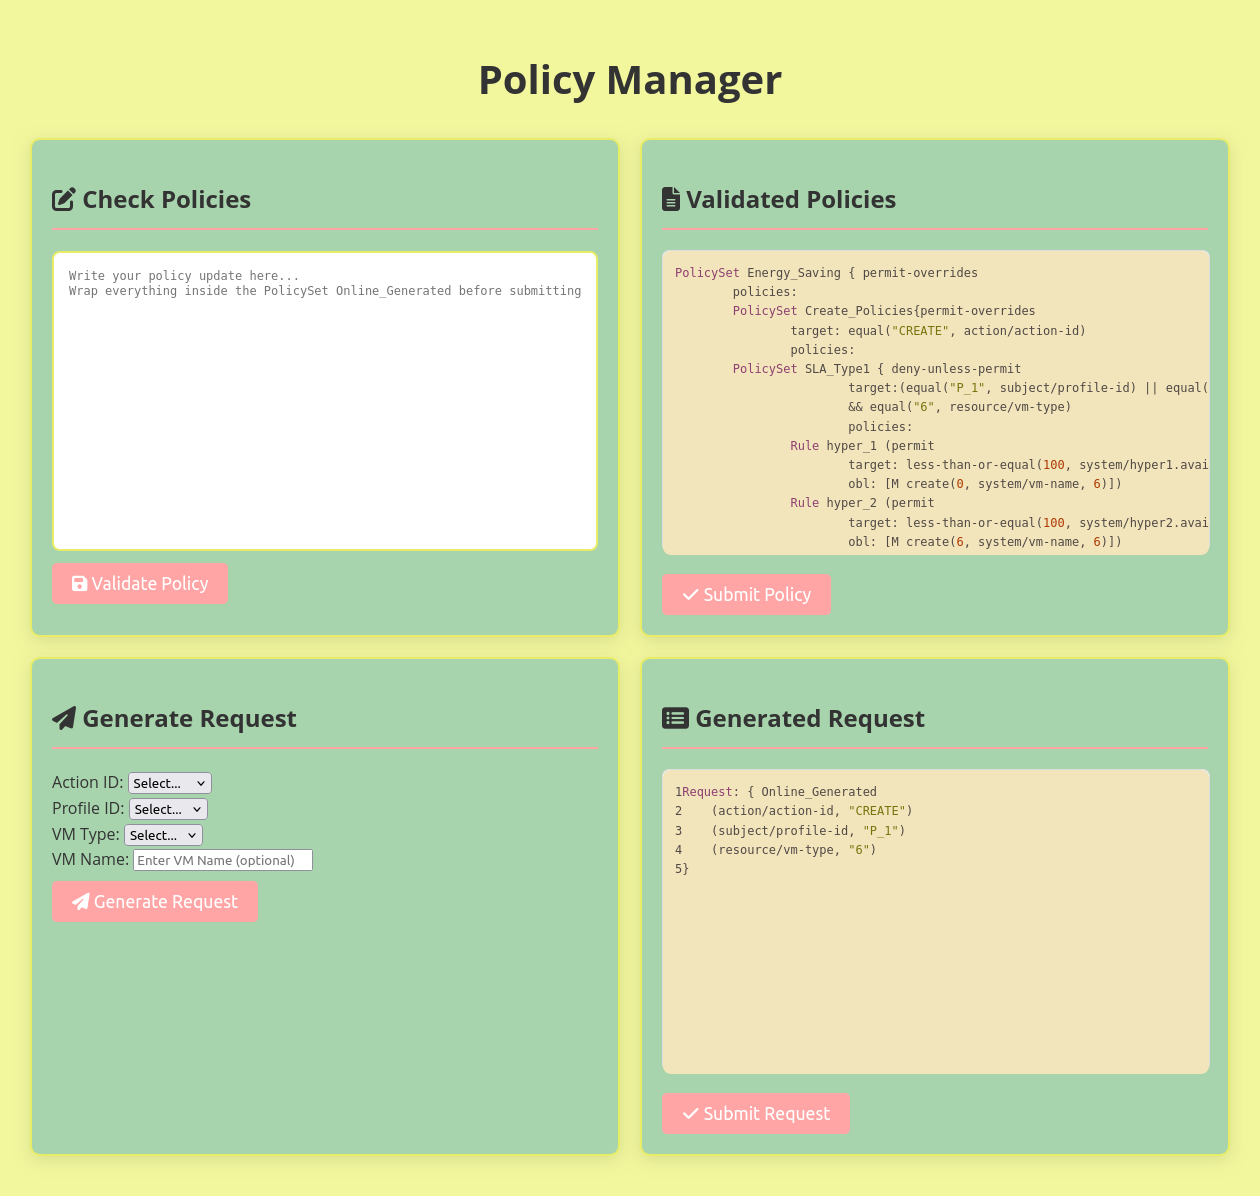
\includegraphics[width=.9\textwidth]{policyManagerFrontEnd}
    \caption{Front-end di policy manager (web app)}
    \label{fig:policyManagerFrontEnd}
    \end{center}
\end{figure}
A livello implementativo si evidenzia l'utilizzo della libreria \emph{highlight.js}\cite{highlightjs} per colorare la sintassi delle policy e delle richieste, questa libreria è stata scelta per la sua semplicità di utilizzo ma anche perchè permette di definire colori personalizzati per ogni linguaggio e anche di aggiungere linguaggi aggiuntivi con uno sforzo minimo grazie all'utilizzo di file JavaScript appositi, come si può leggere dalla documentazione ufficiale\footnote{\url{https://highlightjs.readthedocs.io/en/latest/language-guide.html}}.\medbreak

\section{Sviluppo del backend}
Il backend è stato realizzando sfruttando il framework \emph{Spring Boot}\cite{springboot}, La cui idea di base è quella di semplificare la realizzazione di applicazioni basate su Spring\cite{spring}. Usare Spring Boot Permette di evitare la configurazione manuale di Spring e nel nostro caso ci ha consentito di realizzare un backend per la nostra web app in un modo molto semplice ma comunque modulare. Integrare la logica già descritta nei paragrafi precedenti è stato immediato sia grazie al modo in cui era stato ralizzato il package \texttt{entryPoint} che grazie alla gestione automatica del server web che viene fatta da Spring Boot. In questo esempio infatti le funzionalità di Spring sono state esplorate soltanto in parte ma per il modo in cui è scritto il codice sarà semplice integrare in futuro un database, un servizio di autenticazione o qualunque altro tipo di servizio che si renderà necessario. Inoltre sebbene siano state lasciate le configurazioni di default per springboot e queste fossero sufficienti per il nostro caso di esempio, il framework ha un'ottima documentazione, una grande community e permette di adattarsi a un gran numero di casi concreti.\medbreak
Gli unici due accorgimenti preliminari che sono stati necessari sono stati:
\begin{itemize}
    \item scegliere una versione di Spring Boot compatibile con Java 8: a partire dalla major version 3 infatti, Spring Boot richiede obbligatoriamente una versione di Java 17 o maggiore e quindi la versione da noi è scelta è la 2.7, ovvero l'ultima compatibile con Java 8.
    \item scegliere un framework di logging: di default Spring Boot utilizza logback, ma nel nostro caso abbiamo scelto di usare log4j perchè sia FACPL che Spring utilizzano slf4j come \emph{facade} rendendo impossibile mantenere entrambi i framework di logging. In questo caso risulta più comodo cambiare il framework usato da Spring piuttosto che da FACPL. Per fare questo è stato sufficiente aggiungere la seguente dipendenze al file \texttt{pom.xml}:
    \begin{lstlisting}[language=XML, xleftmargin=1em, caption=Esclusione di logback, label=code:noLogback]
<dependency>
    <groupId>org.springframework.boot</groupId>
    <artifactId>spring-boot-starter-web</artifactId>
    <exclusions>
        <exclusion>
            <groupId>org.springframework.boot</groupId>
            <artifactId>spring-boot-starter-logging</artifactId>
        </exclusion>
    </exclusions>
</dependency>
    \end{lstlisting}
    Grazie a queste righe Spring esclude la dipendenza da logback che è il framework di logging di default e sarà in grado di utilizzare log4j dato che FACPL lega slf4j a log4j. Si evidenzia come questa problematica si presenti solamente nell'ambiente di sviluppo di Eclipse perchè gestisce le dipendenze in modo diverso rispetto a Maven. Utilizzando Maven da terminale il risultato è diverso e viene invece in automatico utilizzato il framework di logging di Spring, tuttavia per rendere il codice facilmente avviabile anche da Eclipse si è deciso di escludere comunque logback e aggiungere invece una dipendeza da log4j di modo che il programma sia avviabile anche da terminale con Maven.
\end{itemize}
Per quanto riguarda le classi che sono state create, si è iniziato creando due \emph{RestController}, ovvero due classi che ricevono chiamate HTTP e sono in grado di dare risposte HTTP, una per le policy e una per le richieste. Queste classi sono state create in modo da rispondere a chiamate POST e GET:
\begin{lstlisting}[language=Java, caption=PolicyController, label=code:PolicyController, basicstyle=\fontsize{10}{11}\ttfamily]
@RestController
@RequestMapping("/policies")
public class PolicyController {
    private final PolicyService policyService;

    @+\mytikzmark{hl1Start}@+public PolicyController(PolicyService policyService) {@+\mytikzmark{hl1End}@+
        @+\mytikzmark{hl2Start}@+this.policyService = policyService;@+\mytikzmark{hl2End}@+
    @+\mytikzmark{hl3Start}@+}@+\mytikzmark{hl3End}@+@+\begin{tikzpicture}[remember picture, overlay]
        \highlight{hl1Start}{hl1End}
        \highlight{hl2Start}{hl2End}
        \highlight{hl3Start}{hl3End}
    \end{tikzpicture}@+

    @GetMapping
    public ResponseEntity<List<String>> getPolicies() throws IOException {
        return policyService.getPolicies();
    }

    @PostMapping("/validate")
    public ResponseEntity<String> validatePolicies(@RequestBody List<String> policies) throws IOException {
        return policyService.validatePolicies(policies);
    }

    @PostMapping("/submit")
    public ResponseEntity<String> submitPolicies() throws IOException {
        return policyService.submitPolicies();
    }
}    
\end{lstlisting}
Il costruttore di questa classe riceve in input un oggetto di tipo \texttt{PolicyService} tuttavia all'interno del progetto non troviamo alcuna chiamata a questo costruttore, questo perchè Spring Boot si occupa di creare un oggetto di tipo \texttt{PolicyService} a partire da un'altra classe che definisce alcuni \texttt{Bean} che verranno poi iniettati nelle classi che li richiedono. I \texttt{Bean} sono oggetti che vengono utilizzati da Spring per passare degli specifici oggetti di un certo tipo in altre classi, in questo caso il \texttt{Bean} di tipo \texttt{PolicyService} è stato definito in una classe chiamata \texttt{ServiceConfig}:
\begin{lstlisting}[language=Java, caption=ServiceConfig, label=code:ServiceConfig]
@Configuration
public class ServiceConfig {
    @Value("${logging.compile.file.name}")
    private String compileLog;
    @Value("${facpl.compile.folderpath}")
    private String compilePath;
    @Bean
    public ApplyPolicy applyPolicy() throws IOException {
        return new ApplyPolicy(compileLog, compilePath);
    }
    @Bean
    public RequestExecution requestExecution() throws IOException {
        return new RequestExecution(compileLog, compilePath);
    }
}
\end{lstlisting}
Le classi \texttt{PolicyController} e \texttt{RequestController} sono sostanzialmente identiche, infatti le richieste da gestire sono le stesse e queste classi non contengono alcun tipo di logica. La logica per la formulazione delle risposte è rimandata alle classi \texttt{PolicyService} e \texttt{RequestService} che a loro volta rimandano buona parte della gestione dei file alle classi presenti nel package \texttt{entryPoint} di \emph{resource\_management}.\medbreak
Per questi motivi anche le due classi \texttt{PolicyService} e \texttt{RequestService} sono molto simili, la parte più interessante di queste classi è sicuramente il metodo per la validazione dei file FACPL, che è stato implementato come segue:
\begin{lstlisting}[language=Java, caption=Metodo validatePolicies, label=code:PolicyServiceValidate, basicstyle=\fontsize{9}{11}\ttfamily]
@Service
public class PolicyService {

@+\mytikzmark{hl1Start}@+@Value("${facpl.policies.filepath}") String policiesFilePath;@+\mytikzmark{hl1End}@+
@+\mytikzmark{hl2Start}@+@Value("${facpl.temp.filepath}") String tempFilePath;@+\mytikzmark{hl2End}@+@+\begin{tikzpicture}[remember picture, overlay]
    \highlight{hl1Start}{hl1End}
    \highlight{hl2Start}{hl2End}
\end{tikzpicture}@+
...
    public ResponseEntity<String> validatePolicies(List<String> policies) throws IOException {
        Files.write(Paths.get(tempFilePath), policies, StandardOpenOption.CREATE, StandardOpenOption.TRUNCATE_EXISTING);
        if (FACPLFileValidator.validate(tempFilePath)) {
            Files.move(Paths.get(tempFilePath), Paths.get(policiesFilePath), StandardCopyOption.REPLACE_EXISTING);
            return ResponseEntity.ok("Valid FACPL file!");
        } else {
            return ResponseEntity.status(HttpStatus.BAD_REQUEST).body("Policy validation failed");
        }
    }
...
}
\end{lstlisting}
Per leggere la posizione di \texttt{policiesFilePath} e \texttt{tempFilePath} è stato utilizzato il file \texttt{application.properties} che è stato inserito nella cartella \emph{src/main/resources} come di default per le applicazioni Spring. Questo lascia la libertà agli utilizzatori di cambiare la posizione dei file senza dover ricompilare il codice. Le posizioni di default sono chiaramente scelte di modo da essere correttamente leggibili e scrivibili da un utente con permessi di lettura e scrittura nella cartella del progetto, quindi nel caso in cui venissero cambiate è necessario assicurarsi che l'utente che lancia l'applicazione abbia i permessi necessari per leggere e scrivere nelle nuove cartelle impostate.\break
Questo metodo riceve da parte del metodo \texttt{getPolicies()} della classe \texttt{PolicyController}, una lista di stringhe che rappresentano le policy, scrive queste stringhe in un file temporaneo e poi chiama il metodo \texttt{validate} della classe \texttt{FACPLFileValidator} che è stato creato appositamente per validare i file FACPL. Questo metodo restituisce un booleano che indica se il file è valido o meno, in caso positivo il file temporaneo viene spostato nella posizione definitiva, altrimenti viene restituito un errore. Si nota inoltre che il return è fatto con un oggetto \texttt{ResponseEntity} che permette di restituire una risposta HTTP con un codice di stato e un corpo, in questo caso il corpo è una stringa che indica se la validazione è andata a buon fine o meno.\medbreak
Nel codice è poi presente una classe \texttt{GlobalExceptionHandler} che grazie alle annotazioni di Spring \texttt{@ControllerAdvice} e \texttt{@ExceptionHandler} permette di gestire le eccezioni che vengono lanciate all'interno del programma, in questo caso vengono gestite le due eccezioni \texttt{Exception} come errore generico e \texttt{IOException} in modo specifico.
\begin{lstlisting}[language=Java, caption=GlobalExceptionHandler, label=code:GlobalExceptionHandler, basicstyle=\fontsize{9.5}{11}\ttfamily]
@ControllerAdvice
public class GlobalExceptionHandler {

    @ExceptionHandler(Exception.class)
    public ResponseEntity<String> handleGeneralException(Exception e) {
        return ResponseEntity.status(HttpStatus.INTERNAL_SERVER_ERROR).body("An unexpected error occurred: " + e.getMessage());
    }

    @ExceptionHandler(IOException.class)
    public ResponseEntity<String> handleIOException(IOException e) {
    	System.out.println("Got catched");
        return ResponseEntity.status(HttpStatus.BAD_REQUEST).body("File processing error: " + e.getMessage());
    }
}
\end{lstlisting}
Il primo metodo restituisce un errore 500, ovvero \texttt{INTERNAL\_SERVER\_ERROR} e il secondo un errore 400, ovvero \texttt{BAD\_REQUEST}. Questa classe è lasciata come esempio di possibile implementazione futura, anche se come si può vedere nel codice delle altre classi la maggior parte delle eccezioni sono gestite singolarmente in questo momento e quindi questa classe non verrà acceduta a meno di errori inattesi. In un'applicazione reale si potrebbe rendere necessario usare questa classe in modo più ampio.

\section{Integrazione della web-app con Maven}
\texttt{policy\_validation}, al contrario di \emph{resource\_management} è stato pensato fin da subito come un progetto Maven e di conseguenza non c'è stato bisogno di alcuna conversione. Spring Boot ha un'integrazione molto semplice con Maven e inoltre, avendo già definito il modo in cui si intendeva integrare dipendenze locali come visto nella sezione \ref{sec:maven}, far funzionare il progetto anche eseguendolo da terminale con Maven è stato immediato.\medbreak
L'unica scelta da prendere riguardava la gestione della dipendenza diretta di \emph{policy\_validation} da \emph{resource\_management}. Una possibilità che è stata presa in considerazione è stata quella di accorpare i due progetti, tuttavia per la natura di \emph{policy\_validation} si è ritenuto che parecchi utenti potrebbero ritenerlo superfluo e quindi che sia meglio mantenere i due progetti separati.\medbreak
Una volta presa questo decisione si è dovuto pensare se fosse opportuno gestire questa dipendenza come tutte le altre dipendenze locali, tuttavia questo avrebbe richiesto diversi passaggi, fra cui la creazione del file .jar di \emph{resource\_management}. La cosa che si è ritenuta più comoda è stata, in questo caso, richiedere di installare il progetto \emph{resource\_management} in locale con Maven, prima di poter utilizzare \emph{policy\_validation}.\medbreak
I due progetti sono quindi pensati per essere distribuiti insieme, ma il primo è completamente indipendente dal secondo, che può essere ignorato o addirittura cancellato se non si intende usarlo. Dato che invece il secondo dipende dal primo e si vuole rendere facile l'applicazione delle modifiche apportate a \emph{resource\_management} di modo che abbiano effetto sul funzionamento di \emph{policy\_validation}, l'unica scelta adatta risulta essere quella presa.

\section{Testing}
Tutte le classi presenti nei due progetti discussi in questi paragrafi presentano delle opportune classi di test. Il framework di test utilizzato è \emph{JUnit5}\cite{junit5} che è stato scelto principalmente per la sua larga diffusione e semplicità di utilizzo.\medbreak
I test per il progetto \emph{resource\_management} sono stati scritti in modo basilare senza utilizzare alcun tipo di framework per la gestione dei Mock. I Mock sono stati comunque necessari date le molte integrazioni con le API di OpenNebula ma si è fatto uso di classi create ad-hoc per il mocking, cosa che ci ha permesso anche di renderci conto più facilmente della testabilità del nostro codice dato che non si è mai fatto ricorso alla reflection di Java.\medbreak
Un esempio di questo è la classe \texttt{CreateVM}, presentata nel listing \ref{code:CreateVM}, la cui classe di test \texttt{CreateVMTest} si presenta nel seguente modo:
\begin{lstlisting}[language=Java, caption=CreateVMTest, label=code:CreateVMTest, basicstyle=\fontsize{9}{10}\ttfamily]
Public class CreateVMTest {

   @+\mytikzmark{hl1Start}@+private StringBuilderLogHandler mockLogHandler;@+\mytikzmark{hl1End}@+@+\begin{tikzpicture}[remember picture, overlay]
    \highlight{hl1Start}{hl1End}
\end{tikzpicture}@+
	private Logger mockLogger;
	
	@BeforeEach
	void setUp() throws ClientConfigurationException {
		mockLogger = Logger.getLogger(CreateVMTest.class.getName());
		mockLogHandler = new StringBuilderLogHandler();
		mockLogger.addHandler(mockLogHandler);
	}
	
    @Test
    public void testEvalSuccess() throws ClientConfigurationException {
    	@+\mytikzmark{hl2Start}@+MockClientTrue mockClient = new MockClientTrue("150");@+\mytikzmark{hl2End}@+@+\begin{tikzpicture}[remember picture, overlay]
            \highlight{hl2Start}{hl2End}\end{tikzpicture}@+
    	MockOpenNebulaActionContext mockContext = new MockOpenNebulaActionContext(mockClient, mockLogger);
    	
        CreateVM createVMAction = new CreateVM(mockContext);

        List<Object> args = Arrays.asList(0, "VMName", 1);
        createVMAction.eval(args);

        assertTrue(mockLogHandler.getLogBuilder().contains("INFO: Starting VM: [1, VMName]\n"));
        assertTrue(mockLogHandler.getLogBuilder().contains("INFO: 150\n"));
    }

    @Test
    public void testEvalFailure() throws ClientConfigurationException {
    	@+\mytikzmark{hl3Start}@+MockClientFalse mockClient = new MockClientFalse("150");@+\mytikzmark{hl3End}@+
    	MockOpenNebulaActionContext mockContext = new MockOpenNebulaActionContext(mockClient, mockLogger);
    	
        CreateVM createVMAction = new CreateVM(mockContext);

        List<Object> args = Arrays.asList(0, "VMName", 1);
        createVMAction.eval(args);;
        
        assertTrue(mockLogHandler.getLogBuilder().contains("INFO: Starting VM: [1, VMName]\n"));
        assertTrue(mockLogHandler.getLogBuilder().contains("SEVERE: 150\n"));
    }
}
\end{lstlisting}
\begin{tikzpicture}[remember picture, overlay]
    \highlight{hl3Start}{hl3End}
\end{tikzpicture}
Quello che possiamo notare è l'utilizzo di tre classi di Mock: \texttt{StringBuilderLogHandler}, \texttt{MockClientTrue} e \texttt{MockClientFalse}. La prima è una classe creata appositamente per il testing che permette di salvare i log in una stringa, le altre due sono classi create per il testing che estendono la classe \texttt{Client} di OpenNebula e che permettono di simulare il comportamento di un client vero e proprio. Queste classi permettono di testare la classe \texttt{CreateVM} in modo indipendente dalla classe \texttt{Client} di OpenNebula, verificando soltanto i side effects delle operazioni, ovvero in questo caso verificando che le stringhe di logging siano coerenti con il comportamento atteso.\medbreak
Per quanto riguarda \emph{policy\_validation} i test sono stati scritti in modo abbastanza diverso, infatti dato che il progetto si basa sul framework Spring Boot si è reso necessario l'utilizzo delle annotazioni specifiche per i test fornite da Spring oltre che il framework \texttt{Mockito}\cite{mockito} per la gestione dei Mock più complessi dove non era necessario avviare l'applicazione Spring Boot. Spring fornisce infatti molte opzioni per il testing, alcune delle quali avviano l'intera app, altre che permettano di inizializzare soltanto il livello web e altre che non hanno proprio bisogno di avviare l'applicazione, il tutto per rendere i test più efficienti e indipendenti dai layer che non sono in fase di test in specifico\footnote{\url{https://docs.spring.io/spring-framework/reference/testing.html}}. Anche in questo caso si evidenzia come queste potenzialità siano state esplorare soltanto sulla superficie data la semplicità della web app in esame.\medbreak
Un esempio di test per il progetto \emph{policy\_validation} sono i test per la classe \texttt{PolicyController}, mostrata nel listing \ref{code:PolicyController}, che si presentano nel seguente modo:
\begin{lstlisting}[language=Java, caption=PolicyControllerTest, label=code:PolicyControllerTest, basicstyle=\fontsize{9}{10}\ttfamily]
@WebMvcTest(PolicyController.class)
class PolicyControllerTest {

    @Autowired
    private MockMvc mockMvc;

    @MockBean
    private PolicyService policyService;

    @Test
    void getPolicies_ShouldReturnPolicyFileContent() throws Exception {
        String policyContent = "Mock Policy Content";
        given(policyService.getPolicies())
            .willReturn(ResponseEntity.ok(Arrays.asList(policyContent)));

        mockMvc.perform(get("/policies"))
                .andExpect(status().isOk())
                .andExpect(content().contentType(MediaType.APPLICATION_JSON))
                .andExpect(content().json("[\"Mock Policy Content\"]"));
    }

    @Test
    void getPolicies_WhenFileNotFound_ShouldReturnNotFound() throws Exception {
        given(policyService.getPolicies())
            .willReturn(ResponseEntity.status(HttpStatus.NOT_FOUND)
                .body(Collections.singletonList("Policies file not found.")));

        mockMvc.perform(get("/policies")
                .accept(MediaType.APPLICATION_JSON))
                .andExpect(status().isNotFound())
                .andExpect(content().contentType(MediaType.APPLICATION_JSON))
                .andExpect(content().json("[\"Policies file not found.\"]"));
    }
    
    @Test
    void validatePolicies_ShouldReturnOk() throws Exception {
        String policyContent = "Mock Policy Content";
        given(policyService.validatePolicies(Arrays.asList(policyContent)))
            .willReturn(ResponseEntity.ok("Validation successful"));

        mockMvc.perform(post("/policies/validate")
                .contentType(MediaType.APPLICATION_JSON)
                .content("[\"Mock Policy Content\"]"))
                .andExpect(status().isOk())
                .andExpect(content().string("Validation successful"));
    }
...
}
\end{lstlisting}
In questo caso si può notare l'utilizzo delle annotazioni \texttt{@WebMvcTest} che permette di caricare soltanto la parte da noi in testing dell'applicazione. Notiamo inoltre l'utilizzo di \texttt{@AutoWired} per iniettare il mock dell'Mvc (\emph{model-view-controller}) di Spring e di \texttt{@MockBean} per iniettare il mock della classe \texttt{PolicyService}. Questo permette di testare la classe \texttt{PolicyController} in modo indipendente dalla classe \texttt{PolicyService} e di verificare che le risposte siano coerenti con il comportamento atteso.\medbreak
Soltano alcuni dei metodi di test sono stati riportati, questo perchè seguono tutti lo stesso schema e differiscono soltanto per i parametri passati e per le risposte attese. Vengono utilizzati \texttt{given} e \texttt{willReturn} per definire il comportamento del mock e successviamente vengono chiamati i metodi \texttt{perform} e \texttt{andExpect} per effettuare la chiamata e verificare che la risposta sia coerente con il comportamento atteso.

\section{Rilascio del progetto}
Come discusso in precedenza, i due progetti sono distribuiti insieme e disponibili alla pagina github \href{https://github.com/alienix2/FACPL_Opennebula_thesis}{\emph{FACPL\_OpenNebula}} con un file README che spiega come installarli e utilizzarli. Questi progetti sono pensati per essere utilizzati da un utente di OpenNebula, quindi l'installazione locale tramite Maven dei progetti deve essere fatta con un utente di questo tipo. Se si cerca di installarlo con un utente che non appartiene a questo gruppo alcuni test falliscono, questo perchè non si riesce ad instanziare nessun oggetto di classe \texttt{Client}. Questo comportamento è voluto e serve a garantire che l'utente che installa il progetto abbia i permessi necessari per utilizzarlo. Nel file README è comunque brevemente indicato un modo per aggirare il problema che consiste nel saltare la fase di test, installare \emph{resource\_management} e avviare quindi tranquillamnte \emph{policy\_validation}, tuttavia affinchè i comandi sulle virtual machine funzionino bisogna per forza avere almeno delle credenziali valide da inserire nella classe \texttt{ContextStub\_Default} e quindi questo metodo è sconsigliato perchè è molto più consono avviare il programma con l'utente corretto.\medbreak
Chiaramente è richiesta all'utente l'installazione di Maven e la presenza di Java 8. L'IDE consigliato per lo sviluppo è Eclipse, non sono stati testati altri IDE ma una volta installati i progetti nel proprio Maven locale, questi sono sicuramente accessibili anche da altri IDE che supportano progetti Maven, includendo le dipendenze nel file \texttt{pom.xml}. Il progetto è testato e funzionante su Ubuntu 20.04, Ubuntu 22.04 e Arch Linux.


\newpage
\section{How did I discover a novel type of heated water}

Explain in detail what are the steps to heat the water in a novel way.

\section{How my heated water differs from the previous ones}

Describe why and how your findings are different from the past versions.

Here you might want to add code (see for example Listing~\ref{code:example}), or tables (see Table~\ref{tab:example}).

Note that figures, listings, tables, and so on, should never be placed `manually'. Let LaTeX decide where to put them - you'll avoid headaches (and bad layouts). Furthermore, each of them must be referred to at least once in the body of the thesis.

\begin{minted}{java}
import java.awt.Rectangle;

public class ObjectVarsAsParameters
{	
    public static void main(String[] args)
    {	go();
    }
    
    public static void go()
    {	
        Rectangle r1 = new Rectangle(0,0,5,5);
        System.out.println("In method go. r1 " + r1 + "\n");
        // could have been 
        //System.out.prinltn("r1" + r1.toString());
        r1.setSize(10, 15);
        System.out.println("In method go. r1 " + r1 + "\n");
        alterPointee(r1);
        System.out.println("In method go. r1 " + r1 + "\n");
        
        alterPointer(r1);
        System.out.println("In method go. r1 " + r1 + "\n");
    }
    
    public static void alterPointee(Rectangle r)
    {	
        System.out.println("In method alterPointee. r " + r + "\n");
        r.setSize(20, 30);
        System.out.println("In method alterPointee. r " + r + "\n");
    }
    
    public static void alterPointer(Rectangle r)
    {	
        System.out.println("In method alterPointer. r " + r + "\n");
        r = new Rectangle(5, 10, 30, 35);
        System.out.println("In method alterPointer. r " + r + "\n");
    }
}
\end{minted}

\begin{lstlisting}[language=Java, caption=Java example, float, label=code:example]
import java.awt.Rectangle;

public class ObjectVarsAsParameters
{	public static void main(String[] args)
    {	go();
    }
    
    public static void go()
    {	Rectangle r1 = new Rectangle(0,0,5,5);
        System.out.println("In method go. r1 " + r1 + "\n");
        // could have been 
        //System.out.prinltn("r1" + r1.toString());
        r1.setSize(10, 15);
        System.out.println("In method go. r1 " + r1 + "\n");
        alterPointee(r1);
        System.out.println("In method go. r1 " + r1 + "\n");
        
        alterPointer(r1);
        System.out.println("In method go. r1 " + r1 + "\n");
    }
    
    public static void alterPointee(Rectangle r)
    {	System.out.println("In method alterPointee. r " + r + "\n");
        r.setSize(20, 30);
        System.out.println("In method alterPointee. r " + r + "\n");
    }
    
    public static void alterPointer(Rectangle r)
    {	System.out.println("In method alterPointer. r " + r + "\n");
        r = new Rectangle(5, 10, 30, 35);
        System.out.println("In method alterPointer. r " + r + "\n");
    }
}
\end{lstlisting}

\begin{table}[tbp]
    \centering
    \caption{Example table}
    \label{tab:example}
    \begin{tabular}{@{}lll@{}}
        \toprule
        Country       & Country code & ISO codes \\ \midrule
        Canada        & 1            & CA / CAN  \\
        Italy         & 39           & IT / ITA  \\
        Spain         & 34           & ES / ESP  \\
        United States & 1            & US / USA  \\ \bottomrule
    \end{tabular}
\end{table}

